\section{Week 2 - Deep convolutional models: case studies}
Learn about the practical tricks and methods used in deep CNNs straight from the research papers.
\subsection{Case studies}

\subsubsection{Why look at case studies?}
It turns out a lot of the past few years of computer vision research has been on how to put together these basic building blocks to form effective convolutional neural networks. Classic networks:
\begin{itemize}
    \item LeNet-5
    \item AlexNet
    \item VGG
\end{itemize}
Other NN: ResNet (152) layers, Inception network

\subsubsection{Classic Networks}
History of Deep learning networks.

\subsubsection{ResNet}
Residual Networks: are based on Residual Blocks where the activation of a layer is used again further deep in the network (creating \textbf{Shortcut} / \textbf{Skip connections}):
\begin{equation*}
z^{[l+1]} = W^{[l+1]} a^{[l]} + b^{[l+1]} => a^{[l+1]} = g(z^{[l+1]}) => z^{[l+2]} = W^{[l+2]} a^{[l+1]} + b^{[l+2]} => a^{[l+2]} = g(z^{[l+2]})
\end{equation*}
Then reuse $a^{[l]}$ again in $a^{[l+2]}$, so the later becomes:
\begin{equation*}
a^{[l+2]} = g(z^{[l+2]}  + a^{[l]}) 
\end{equation*}
In theory as we increase the number of hidden layers the NN does better and better. However, in practice it does well until a certain number of hidden NN after that the performance goes down. \textbf{ResNet} allows you build deep NN (e.g. thousands of hidden layers) while keep improving the performance.


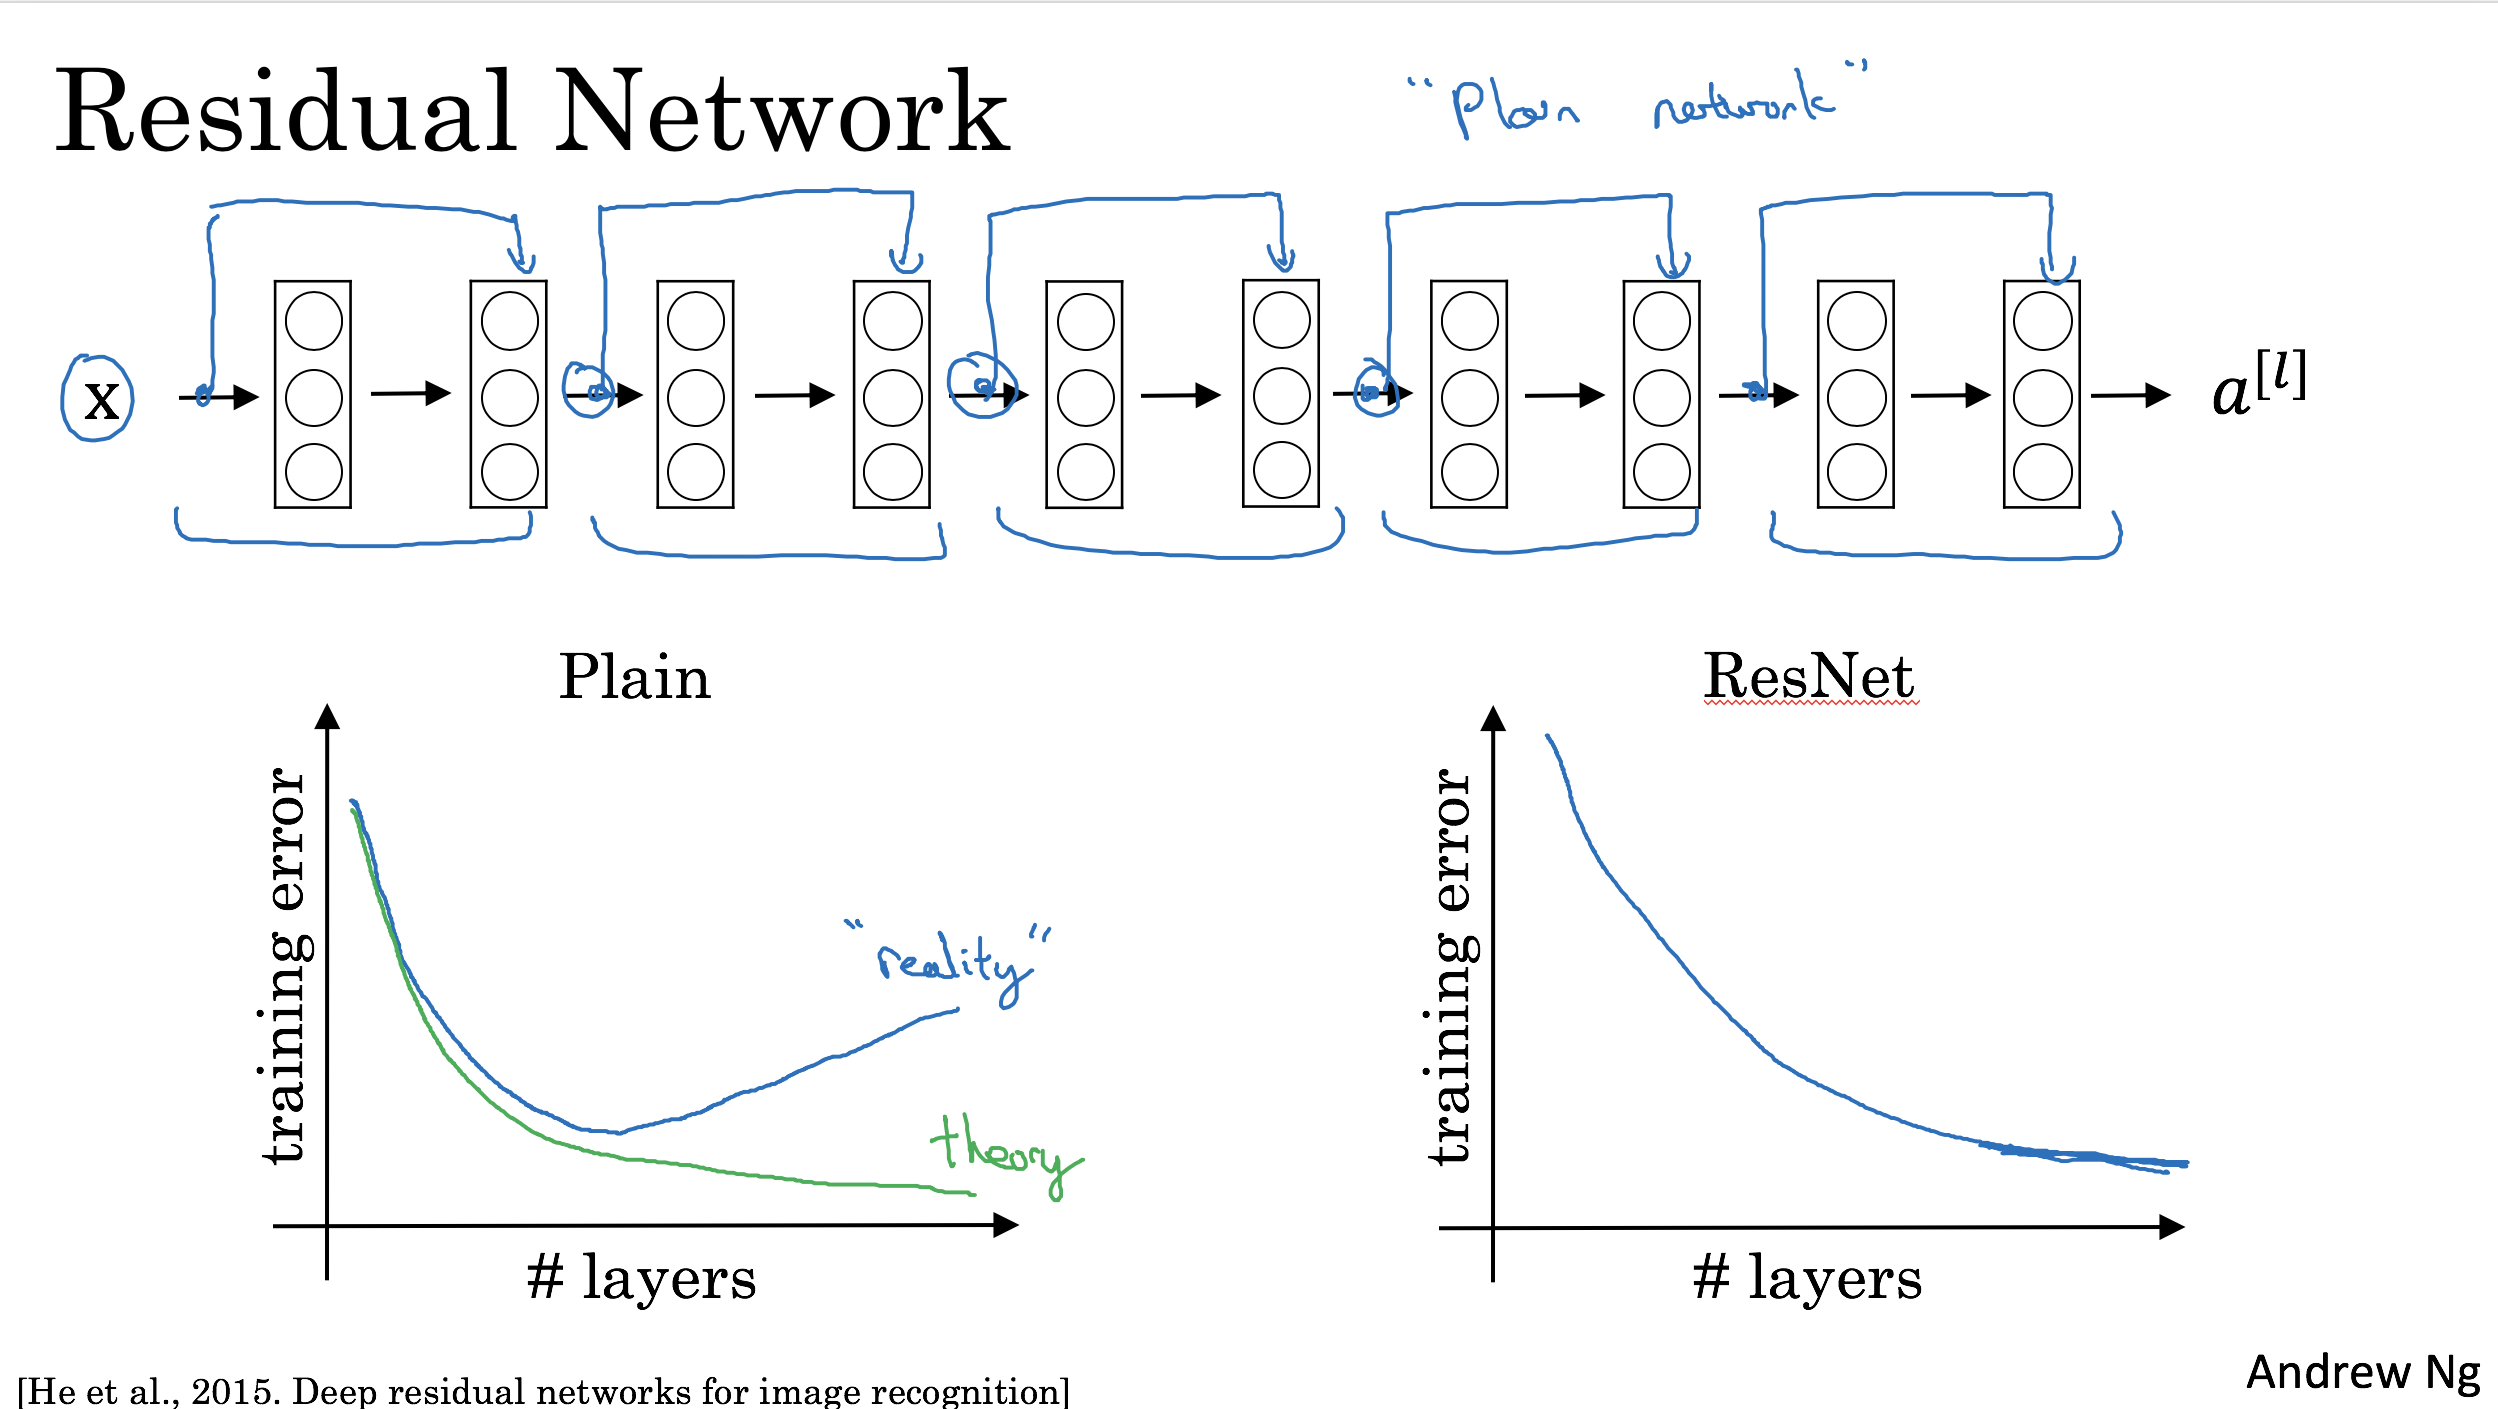
\includegraphics[scale=0.35]{ResNet}

\subsubsection{Why ResNets Work}

\subsubsection{Networks in Networks and 1x1 Convolutions}
It is basically multiplying the input matrix by 2, this is in case of one channel. But in case of multiple channels, it's useful to shrunk the number of channels.
1x1 convolution is also called network in network.

\subsubsection{Inception Network Motivation}
Reducing the number of channels with a \textbf{Bottleneck} layer which performs a 1x1 convolution:


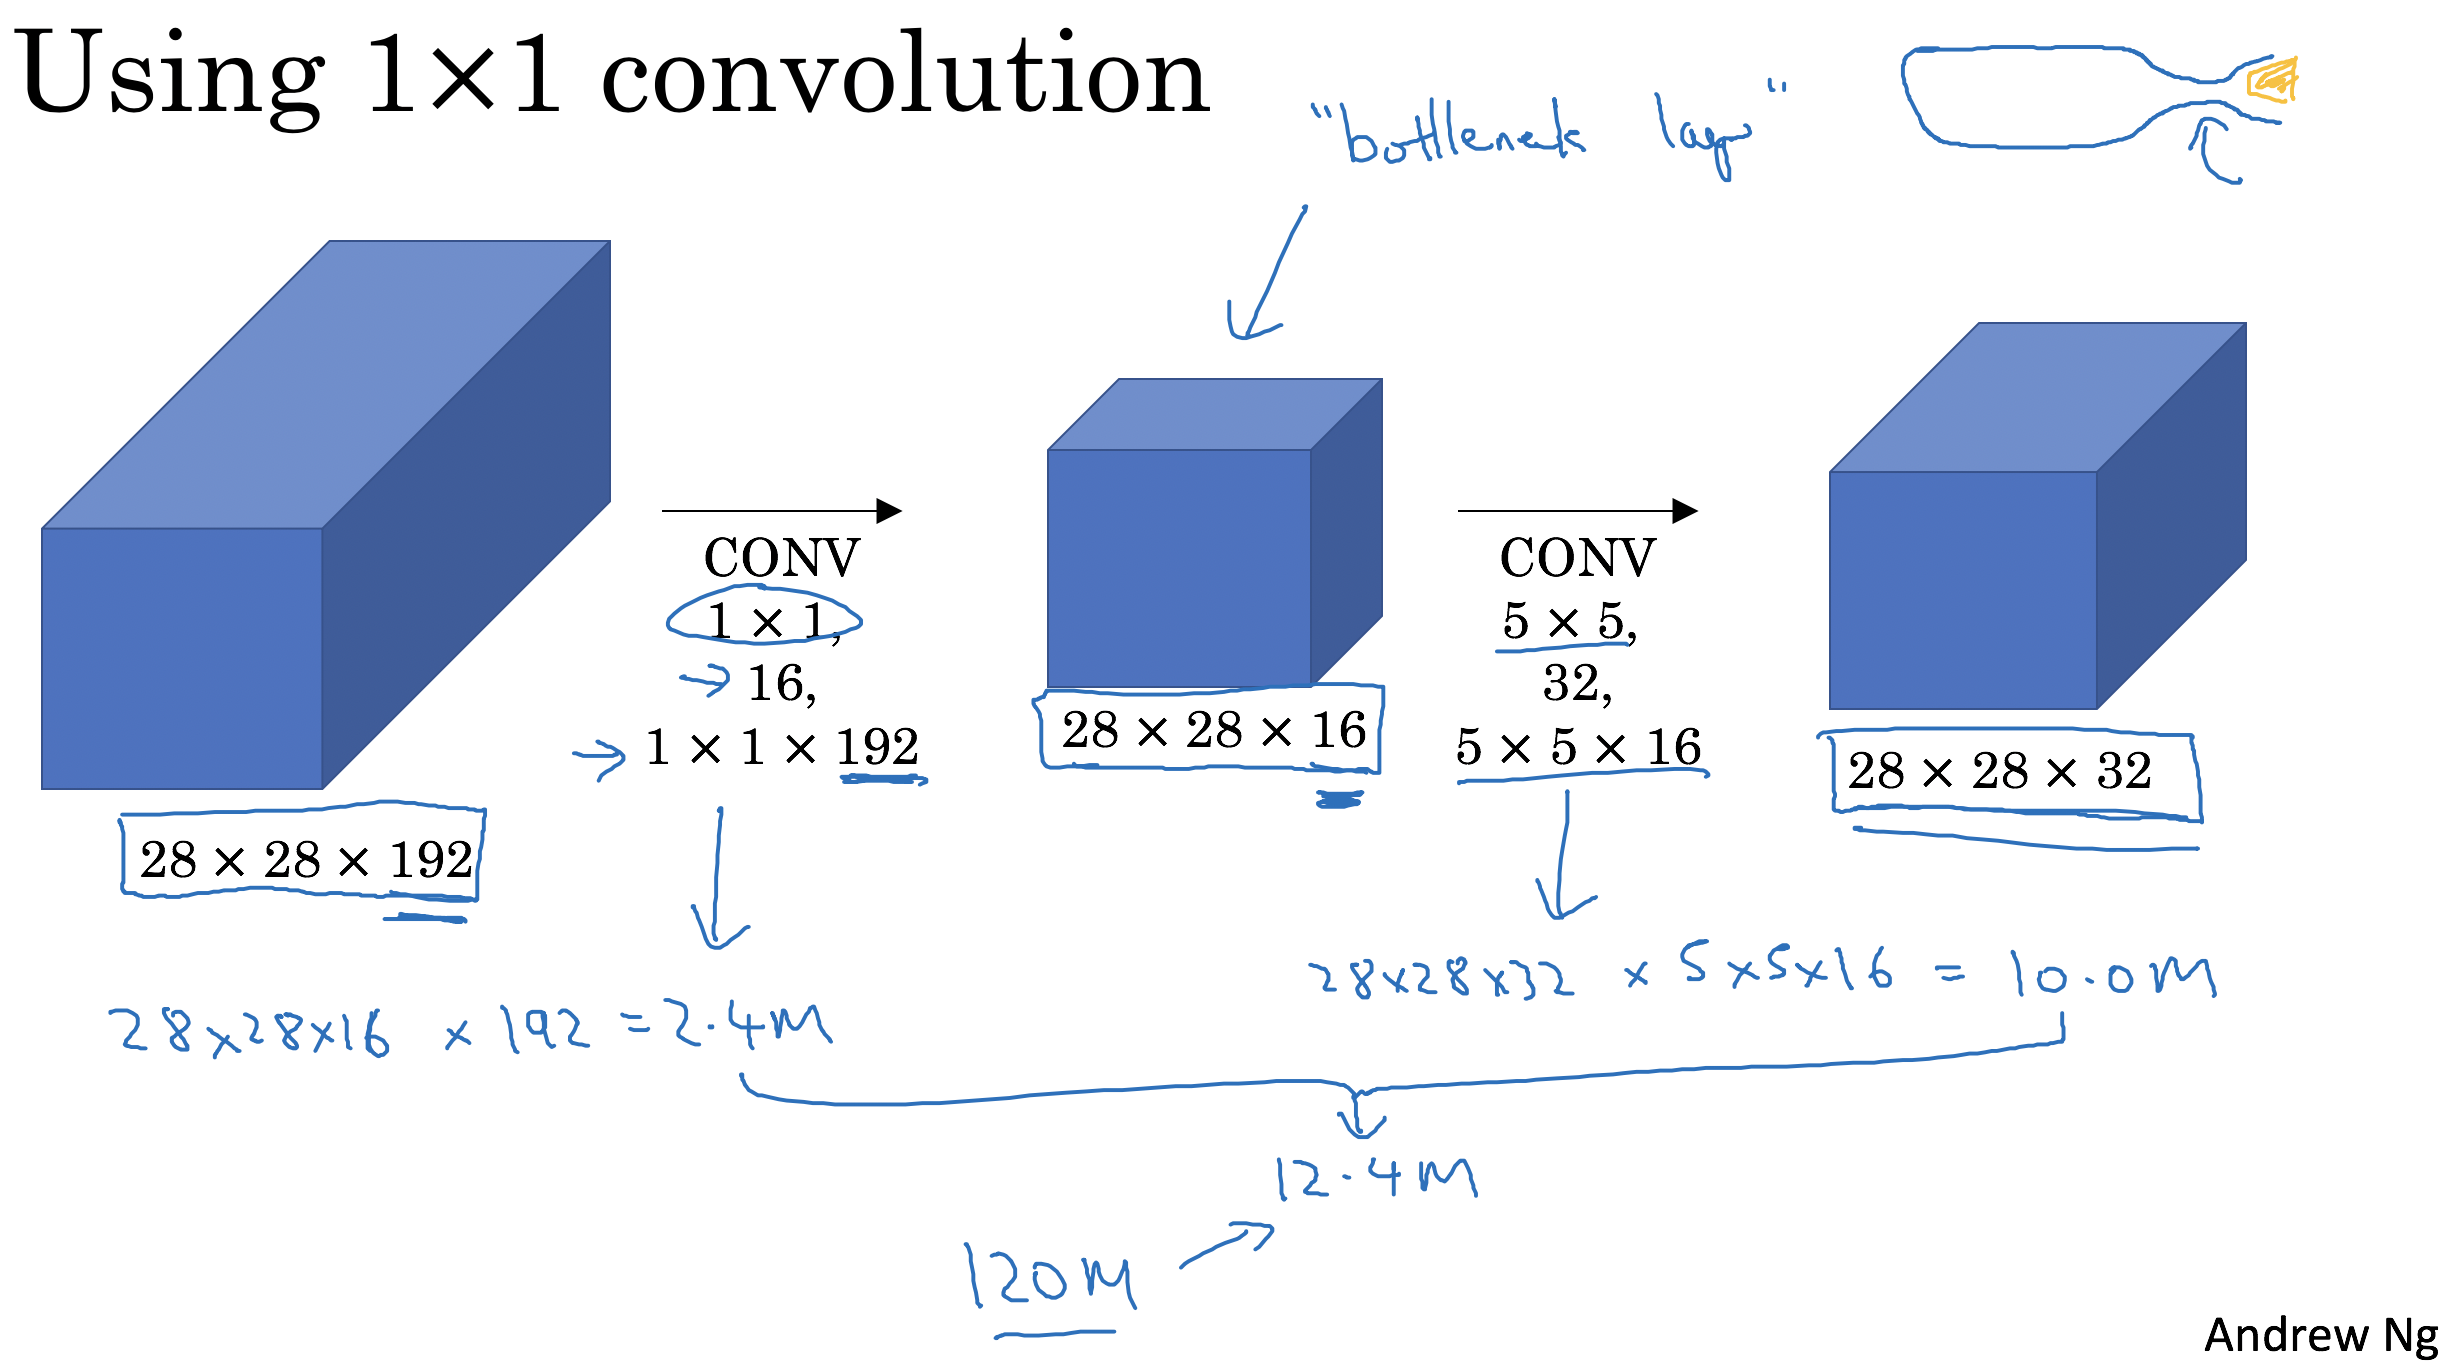
\includegraphics[scale=0.35]{InceptionNet_motivation}

\subsubsection{Inception Network}
Similar to ResNet, Inception Net are based on Inception block that are chained together to create a complete net. It also contains side branches to predict the output directly from the the hidden / intermediate networks.


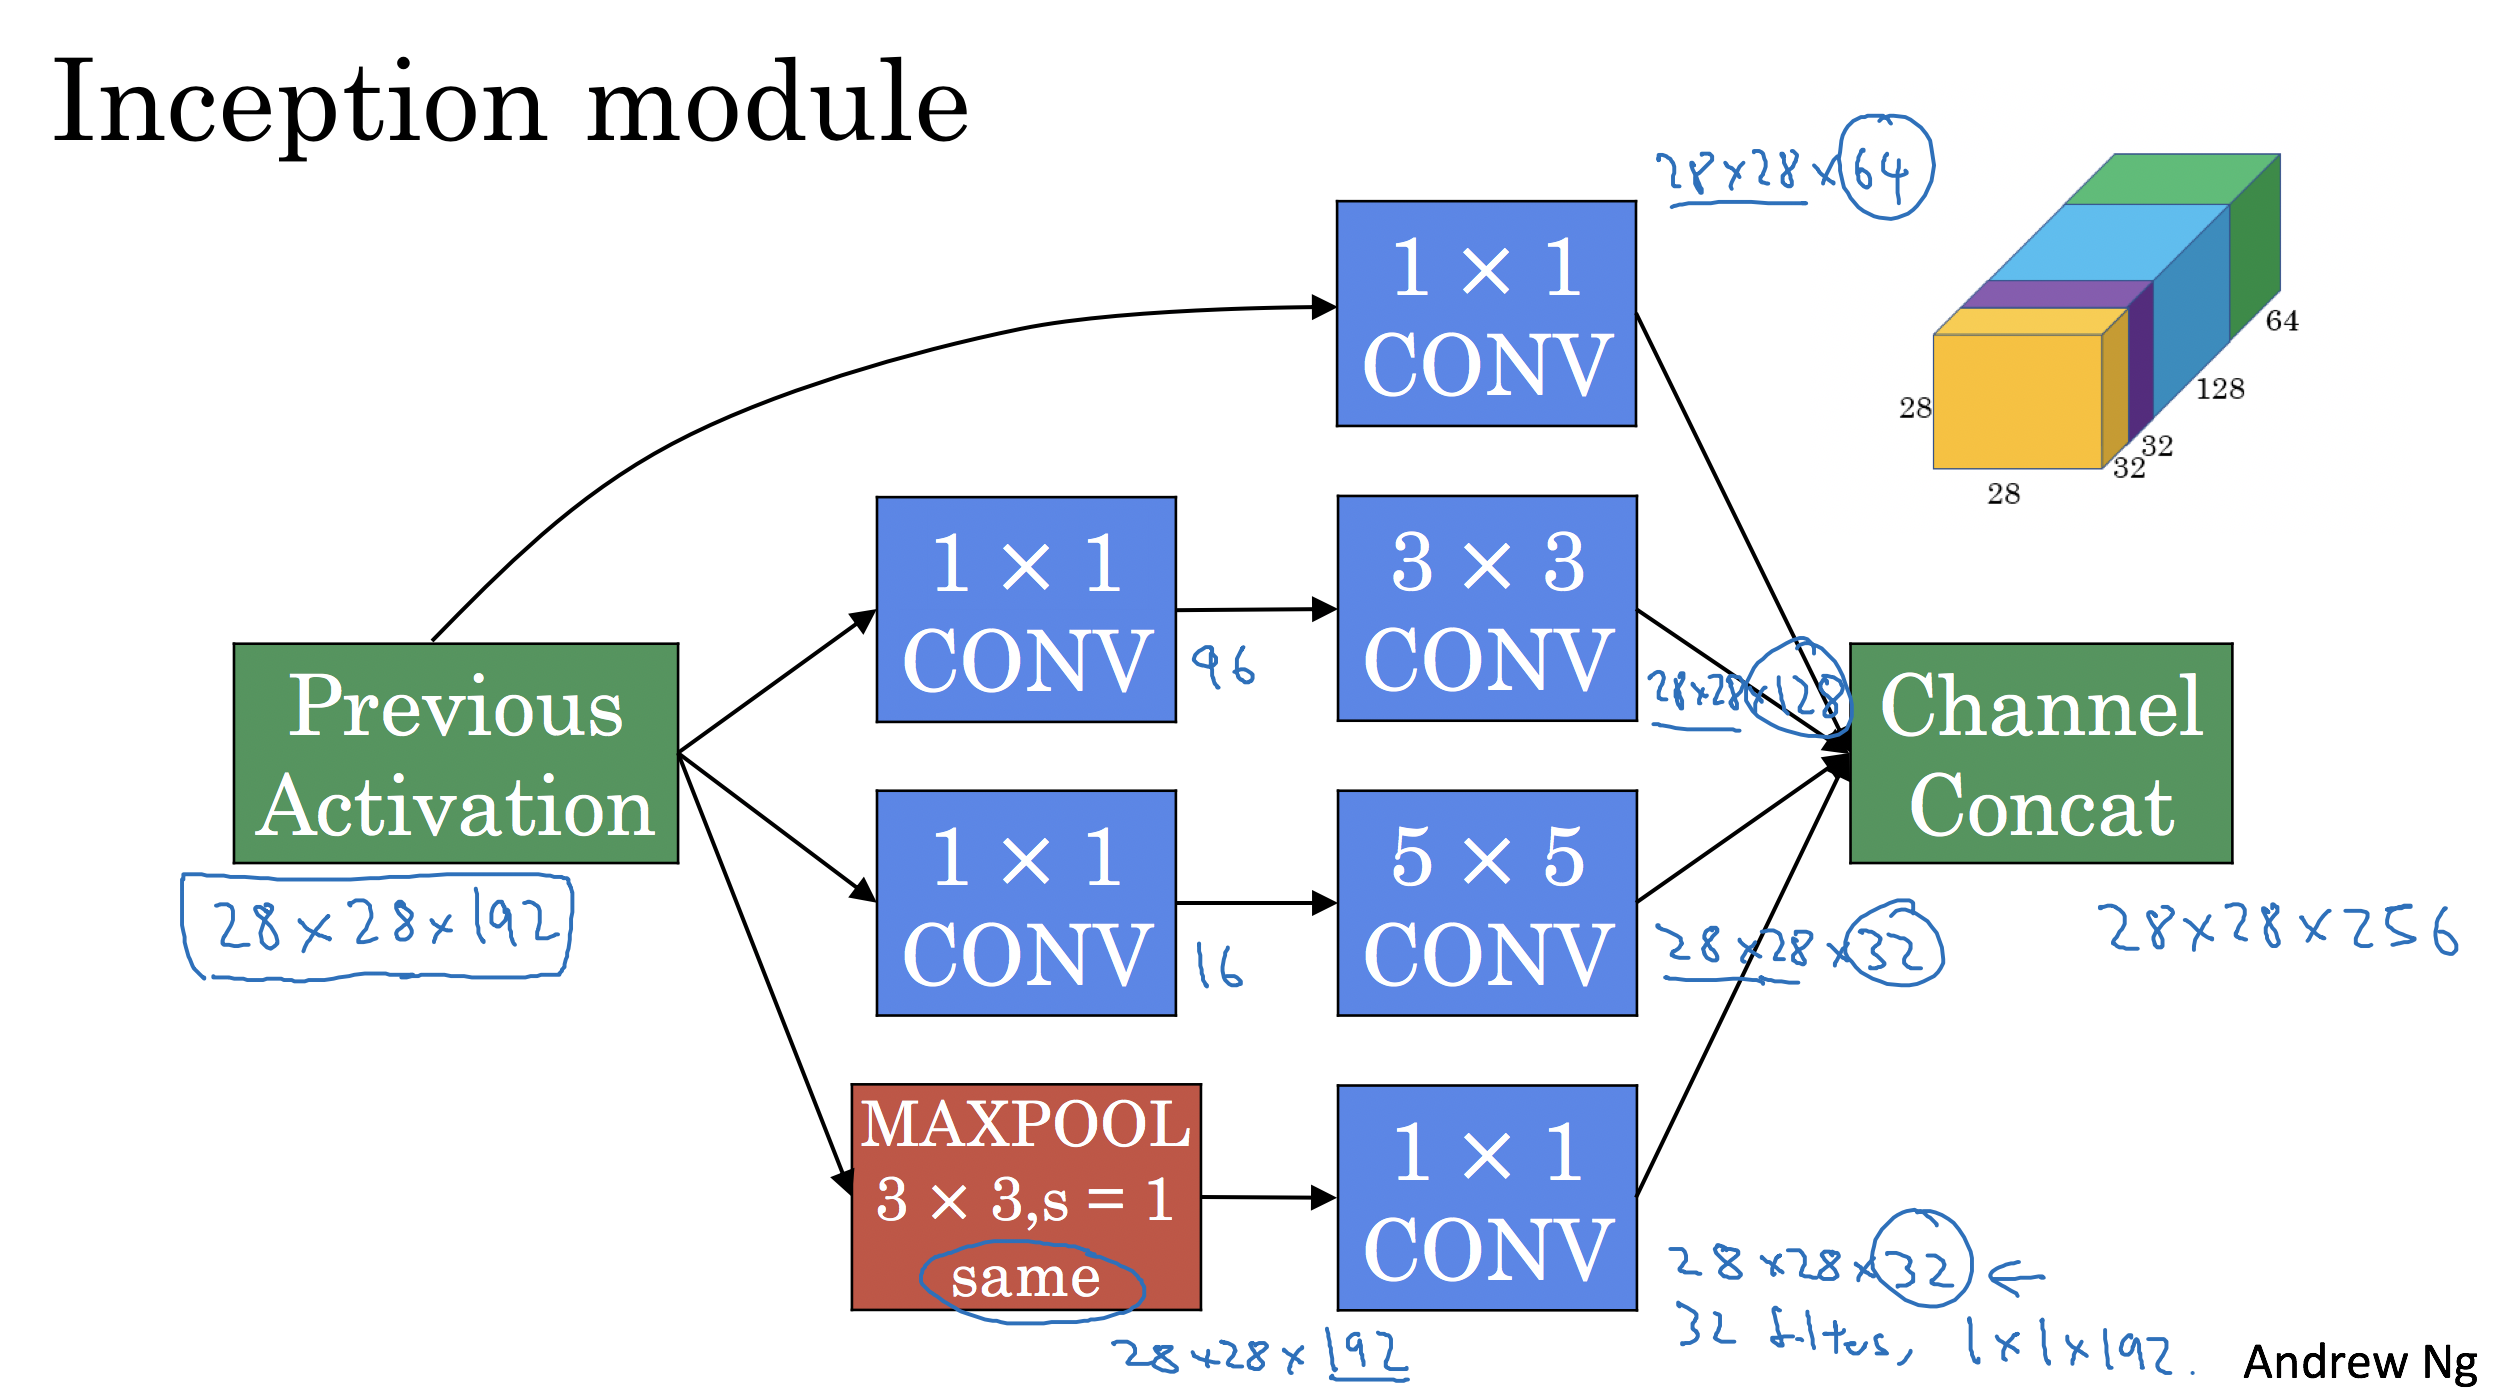
\includegraphics[scale=0.35]{Inception_block}

\subsection{Practical advices for using ConvNets}

\subsubsection{Using Open-Source Implementation}
Pratcial advices on using the NN seeing in the previous videos.
If you're developing a computer vision application, a very common workflow would be to: 
\begin{itemize}
    \item pick an architecture that you like, (e.g. from those learned in this course) or one that you heard about from a friend or from some literature. 
    \item And look for an open source implementation and download it from GitHub to start building from there.
\end{itemize}
One of the advantages of doing so also is that sometimes these networks take a long time to train (e.g. multiple GPUs, very large dataset to pretrain). And that allows you to do transfer learning using these networks. 

\subsubsection{Transfer Learning}
When building a computer vision application, rather than training the ways from scratch, from random initialization, you often make much faster progress if you download ways that someone else has already trained on the network architecture and use that as pre-training and transfer that to a new task that you might be interested in.

You can often download open source ways that took someone else many weeks or months to figure out and use it to initialize your NN.

\subsubsection{Data Augmentation}
Common augmentation method:
\begin{itemize}
    \item Mirroring: e.g. mirror a picture on the vertical axes
    \item Random cropping: unless the cropped picture preserve properties of the original, e.g. Cropping the background in a cat picture is not a cat.
    \item color shifting: motivation if the sunlight is yellow or illumination, e.g. color distortion: changing red by green.
    \item Advanced color augmentation: PCA color augmentation: (in AlexNet paper)
\end{itemize}
Implementing distortions during training.

\subsubsection{State of Computer Vision}
Tips for doing well on benchmarks/winning competitions (not for production systems):
\begin{itemize}
    \item \textbf{Ensembling:} Train serval networks (e.g. 3 to 15 NN) independently and average their outputs (i.e. average $\hat{y}$ not the weights)
    \item \textbf{Multi-crop at test time:} Run classifier on multiple vertions of test images and average results
\end{itemize}
Use open source code:
\begin{itemize}
    \item Use architectures of networks published in the literature
    \item Use open source implementations if possible
    \item Use pretrained models and fine-tune on your dataset
\end{itemize}

\subsection{Practice questions}

\subsubsection{QUIZ - Deep convolutional models}
\textbf{1.} Which of the following do you typically see as you move to deeper layers in a ConvNet?
\begin{itemize}
    \item $n_H$ and $n_W$ increases, while $n_C$ also increases
    \item $n_H$ and $n_W$ decrease, while $n_C$ increases (X)
    \item $n_H$ and $n_W$ increases, while $n_C$ decreases
    \item $n_H$ and $n_W$ decreases, while $n_C$ also decreases
\end{itemize}
\textbf{2.} Which of the following do you typically see in a ConvNet? (Check all that apply.)
\begin{itemize}
    \item Multiple CONV layers followed by a POOL layer (X)
    \item Multiple POOL layers followed by a CONV layer
    \item FC layers in the last few layers (X)
    \item FC layers in the first few layers
\end{itemize}
\textbf{3.} In order to be able to build very deep networks, we usually only use pooling layers to downsize the height/width of the activation volumes while convolutions are used with “valid” padding. Otherwise, we would downsize the input of the model too quickly.
\begin{itemize}
    \item True (X 1)
    \item False (X 2)
\end{itemize}
\textbf{4.} Training a deeper network (for example, adding additional layers to the network) allows the network to fit more complex functions and thus almost always results in lower training error. For this question, assume we’re referring to “plain” networks.
\begin{itemize}
    \item True
    \item False (X)
\end{itemize}
\textbf{5.} The following equation captures the computation in a ResNet block. What goes into the two blanks above?
\begin{equation*}
    a^{[l+2]}=g(W^{[l+2]}g(W^{[l+1]})a^{[l]}+b^{[l+1]})+b^{l+2}+\_\_\_\_\_\_\_ )+\_\_\_\_\_\_\_
\end{equation*}
\begin{itemize}
    \item 0 and $a^{[l]}$, respectively
    \item $a^{[l]}$ and 0, respectively (X)
    \item 0 and $z^{[l+1]}$, respectively
    \item $z^{[l]}$ and $a^{[l]}$, respectively
\end{itemize}
\textbf{6.} Which ones of the following statements on Residual Networks are true? (Check all that apply.)
\begin{itemize}
    \item The skip-connection makes it easy for the network to learn an identity mapping between the input and the output within the ResNet block. (X)
    \item The skip-connections compute a complex non-linear function of the input to pass to a deeper layer in the network.
    \item A ResNet with L layers would have on the order of $L^2$  skip connections in total.
    \item Using a skip-connection helps the gradient to backpropagate and thus helps you to train deeper networks (X)
\end{itemize}
\textbf{7.} Suppose you have an input volume of dimension 64x64x16. How many parameters would a single 1x1 convolutional filter have (including the bias)?
\begin{itemize}
    \item 2
    \item 1
    \item 4097
    \item 17 (X)
\end{itemize}
\textbf{8.} Suppose you have an input volume of dimension $n_H$ x $n_W$ x $n_C$ . Which of the following statements you agree with? (Assume that “1x1 convolutional layer” below always uses a stride of 1 and no padding.)
\begin{itemize}
    \item You can use a 1x1 convolutional layer to reduce $n_C$ but not $n_H$, $n_W$. (X)
    \item You can use a 1x1 convolutional layer to reduce $n_H$, $n_W$, and $n_C$.
    \item You can use a pooling layer to reduce $n_H$, $n_W$, but not $n_C$. (X)
    \item You can use a pooling layer to reduce $n_H$, $n_W$, and $n_C$.
\end{itemize}
\textbf{9.} Which ones of the following statements on Inception Networks are true? (Check all that apply.)
\begin{itemize}
    \item Inception networks incorporates a variety of network architectures (similar to dropout, which randomly chooses a network architecture on each step) and thus has a similar regularizing effect as dropout.
    \item Inception blocks usually use 1x1 convolutions to reduce the input data volume’s size before applying 3x3 and 5x5 convolutions. (X)
    \item A single inception block allows the network to use a combination of 1x1, 3x3, 5x5 convolutions and pooling. (X)
    \item Making an inception network deeper (by stacking more inception blocks together) should not hurt training set performance. (X)
\end{itemize}
\textbf{10.} Which of the following are common reasons for using open-source implementations of ConvNets (both the model and/or weights)? Check all that apply.
\begin{itemize}
    \item Parameters trained for one computer vision task are often useful as pretraining for other computer vision tasks. (X)
    \item The same techniques for winning computer vision competitions, such as using multiple crops at test time, are widely used in practical deployments (or production system deployments) of ConvNets.
    \item It is a convenient way to get working an implementation of a complex ConvNet architecture. (X)
    \item A model trained for one computer vision task can usually be used to perform data augmentation even for a different computer vision task.
\end{itemize}